%=============================================================
%  PRESENTACIÓN — DEFENSA DE TESINA
%  Magíster en Ciencia de Datos para la Innovación, UdeC
%  Compilar con: XeLaTeX
%=============================================================
\documentclass[10pt, aspectratio=169]{beamer}

\usetheme{metropolis}

\usepackage{fontspec}
\usepackage{polyglossia}
\setmainlanguage{spanish}

\usepackage{graphicx}
\usepackage{booktabs}
\usepackage{amsmath}
\usepackage{xcolor}

%-------------------------------------------------------------
%  PALETA — OPCIÓN C: NOCHE Y CIAN
%-------------------------------------------------------------
\definecolor{primary}{HTML}{0D1B2A}
\definecolor{accent}{HTML}{00B4A6}
\definecolor{softbg}{HTML}{F4F6F7}
\definecolor{mutedtext}{HTML}{4A5568}

\setbeamercolor{normal text}         {fg=primary,   bg=white}
\setbeamercolor{alerted text}        {fg=accent}
\setbeamercolor{example text}        {fg=accent!80!primary}
\setbeamercolor{frametitle}          {bg=primary,   fg=white}
\setbeamercolor{progress bar}        {fg=accent,    bg=primary!30}
\setbeamercolor{title separator}     {fg=accent}
\setbeamercolor{palette primary}     {bg=primary,   fg=white}
\setbeamercolor{block title}         {bg=primary!8, fg=primary}
\setbeamercolor{block body}          {bg=softbg}
\setbeamercolor{block title alerted} {bg=accent!15, fg=primary}
\setbeamercolor{block body alerted}  {bg=accent!5}

\setbeamerfont{title}      {size=\large,      series=\bfseries}
\setbeamerfont{subtitle}   {size=\small,      series=\normalfont}
\setbeamerfont{frametitle} {size=\normalsize, series=\bfseries}
\setbeamerfont{block title}{series=\bfseries}

\metroset{progressbar=frametitle, block=fill}

\newcommand{\hl}[1]{\textcolor{accent}{\textbf{#1}}}
\newcommand{\emp}[1]{\textcolor{primary}{\textbf{#1}}}

%-------------------------------------------------------------
%  METADATA
%-------------------------------------------------------------
\titlegraphic{%
	
\includegraphics[height=0.9cm]{logos/logo_mag.png}%
	\hfill%
	
\includegraphics[height=0.9cm]{logos/logo_cdia.png}%
}
\title{Estimación de Variables Geometalúrgicas\\con Machine Learning}
\subtitle{Defensa de Tesina}
\author{Ignacio Enrique Rojas Rodríguez}
\institute{%
	Magíster en Ciencia de Datos para la Innovación\\
	Universidad de Concepción\\[3pt]
	{\footnotesize\textcolor{mutedtext}{%
			Profesor guía: Pedro Pinacho \enspace|\enspace
			Profesor co-guía: José Ulloa}}
}
\date{Marzo de 2026}

%=============================================================
\begin{document}
	%=============================================================
	
	\begin{frame}[plain]
		\titlepage
	\end{frame}
	
	\begin{frame}{Agenda}
		\tableofcontents
	\end{frame}
	
	%=============================================================
	\section{Contexto y problema}
	%=============================================================
	
	\begin{frame}{La geometalurgia y el desafío de los datos}
		\begin{columns}[T]
			\begin{column}{0.55\textwidth}
				\textbf{¿Qué es la geometalurgia?}\\[4pt]
				Disciplina que vincula las \hl{características geológicas} de un
				yacimiento con su \hl{respuesta metalúrgica} en el proceso de beneficio.\\[10pt]
				
				\textbf{El problema central: asimetría de datos}
				\begin{itemize}
					\item Datos geológicos → \emp{abundantes} (sondajes extensos)
					\item Datos geometalúrgicos → \emp{escasos} (ensayos de laboratorio costosos)
				\end{itemize}
			\end{column}
			\begin{column}{0.42\textwidth}
				\begin{block}{Recuperación en peso}
					Variable objetivo del estudio:\\[6pt]
					\[
					R_p(\%) = \frac{Masa_{Conc}}{Masa_{Alim}} \times 100
					\]
					{\small Razón entre la masa del concentrado
						obtenido y la masa total alimentada.}
				\end{block}
			\end{column}
		\end{columns}
	\end{frame}
	
	\begin{frame}{Limitaciones del enfoque tradicional}
		\begin{columns}[T]
			\begin{column}{0.48\textwidth}
				\textbf{Kriging — método oficial}
				\begin{itemize}
					\item Robusto con alta densidad de muestreo
					\item Con datos escasos requiere:
					\begin{itemize}
						\item Juicio experto intensivo
						\item Supuestos de estacionariedad
						\item Modelado variográfico iterativo
					\end{itemize}
					\item Depende de \hl{software propietario de alto costo}
				\end{itemize}
			\end{column}
			\begin{column}{0.48\textwidth}
				\begin{alertblock}{Hipótesis}
					Los algoritmos de Machine Learning poseen
					la flexibilidad para capturar relaciones
					espaciales complejas \textbf{sin} las rígidas
					restricciones paramétricas de la
					geoestadística tradicional.
				\end{alertblock}
			\end{column}
		\end{columns}
	\end{frame}
	
	%=============================================================
	\section{Propuesta y objetivos}
	%=============================================================
	
	\begin{frame}{Descripción de la propuesta}
		\begin{columns}[T]
			\begin{column}{0.48\textwidth}
				\begin{block}{MVP en Python}
					Pipeline automatizado que ejecuta de principio a fin:
					\begin{itemize}
						\item Carga y limpieza de datos
						\item Análisis exploratorio (EDA)
						\item Domaining no supervisado
						\item Entrenamiento de modelos supervisados
						\item Estimación masiva sobre modelo de bloques
					\end{itemize}
				\end{block}
			\end{column}
			\begin{column}{0.48\textwidth}
				\textbf{Tres dimensiones clave}\\[6pt]
				\hl{Técnica} — Capturar continuidad espacial\\
				con métricas de error competitivas\\[8pt]
				\hl{Negocio} — Reducir tiempos y costos\\
				de software propietario\\[8pt]
				\hl{Adopción} — Código base replicable\\
				que democratiza el análisis de datos
			\end{column}
		\end{columns}
	\end{frame}
	
	\begin{frame}{Objetivos}
		\textbf{Objetivo general}\\[4pt]
		Desarrollar y evaluar un flujo de trabajo basado en ML para la
		\hl{estimación espacial de variables geometalúrgicas con datos escasos},
		contrastando su rendimiento frente a las metodologías geoestadísticas
		tradicionales.\\[12pt]
		
		\textbf{Objetivos específicos}
		\begin{enumerate}
			\item Diseñar un flujo automatizado de preprocesamiento y transformación estadística
			\item Implementar K-Means para la delimitación de dominios geometalúrgicos espaciales
			\item Entrenar y optimizar modelos supervisados para predecir la recuperación en peso
			\item Comparar desempeño cuantitativo y coherencia espacial del ML vs Kriging
		\end{enumerate}
	\end{frame}
	
	%=============================================================
	\section{Datos y depuración}
	%=============================================================
	
	\begin{frame}{Fuentes de datos}
		\begin{columns}[T]
			\begin{column}{0.48\textwidth}
				\begin{block}{Base de laboratorio}
					\begin{itemize}
						\item 1.219 registros válidos de ensayos geometalúrgicos
						\item Variables: coordenadas 3D (Este, Norte, Cota) + recuperación en peso (\%)
						\item Fuente externa — datos confidenciales
					\end{itemize}
				\end{block}
			\end{column}
			\begin{column}{0.48\textwidth}
				\begin{block}{Modelo de bloques (benchmark)}
					\begin{itemize}
						\item 343.732 puntos estimados mediante \emp{Kriging}
						\item Construido con la misma base de laboratorio
						\item Rol exclusivo: \hl{validación externa} del MVP
					\end{itemize}
				\end{block}
			\end{column}
		\end{columns}
	\end{frame}
	
	\begin{frame}{Depuración y transformación}
		\begin{columns}[T]
			\begin{column}{0.38\textwidth}
				\textbf{Limpieza de datos}\\[6pt]
				\begin{itemize}
					\item 1.466 registros originales
					\item $-$ 230 con valor \texttt{-99}
					\item $-$ 17 fuera del área de interés
					\item[\textbf{=}] \hl{1.219 registros válidos} (83,2\%)
				\end{itemize}
				\vspace{8pt}
				\textbf{Normal Score Transformation}\\[4pt]
				Ajusta la distribución original a\\
				normal estándar ($\mu=0$, $\sigma=1$).\\[4pt]
				Todo el modelado se realizó sobre\\
				la \emp{variable transformada}.
			\end{column}
			\begin{column}{0.60\textwidth}
				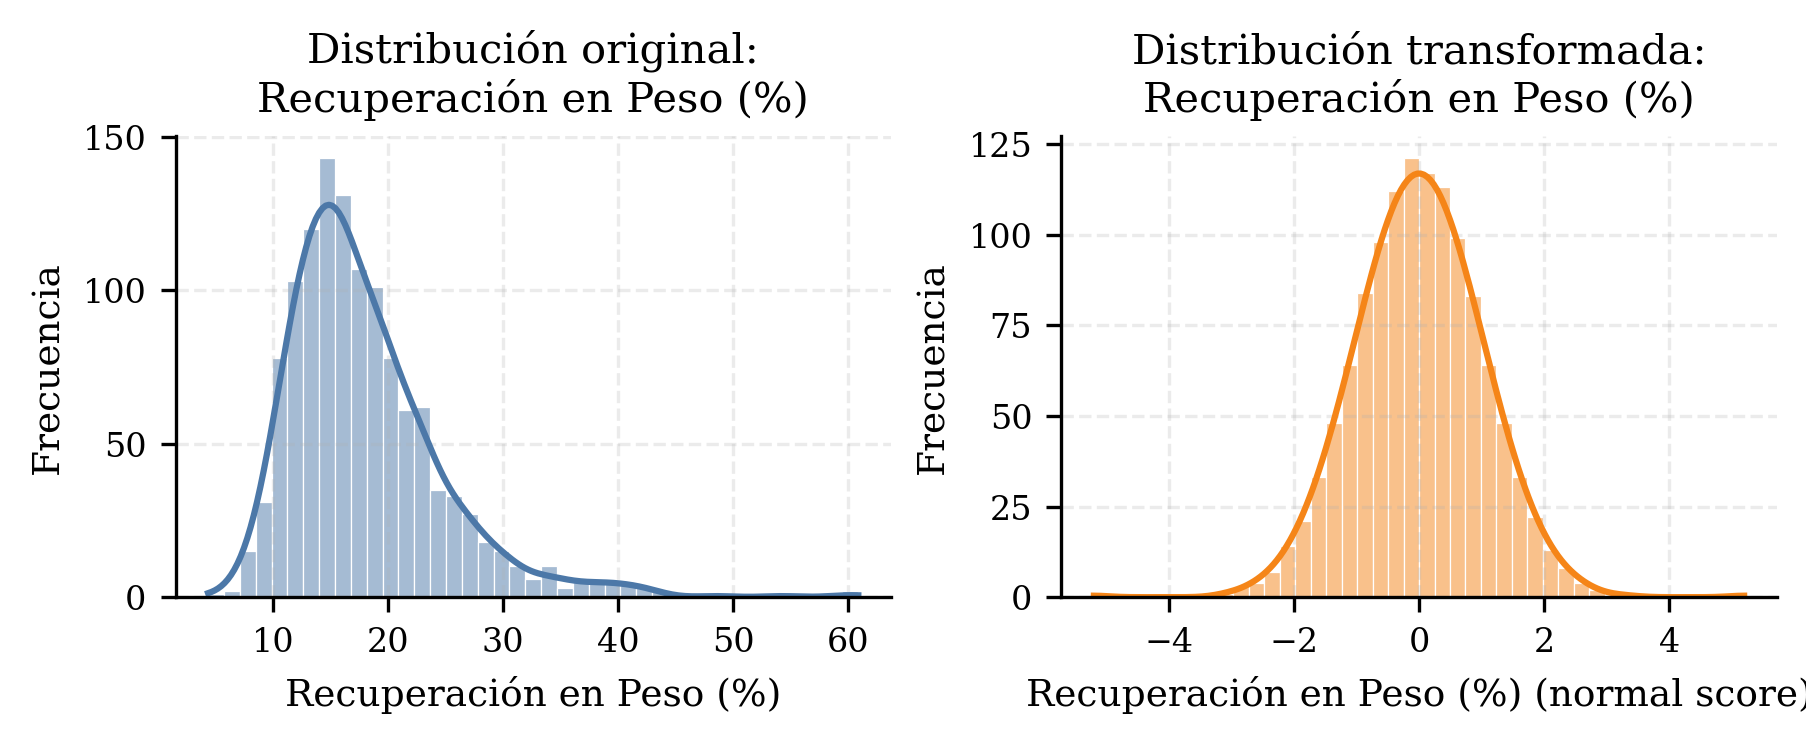
\includegraphics[width=\textwidth]{Imagenes/hist_original_vs_gauss_recpe.png}
			\end{column}
		\end{columns}
	\end{frame}
	
	%=============================================================
	\section{Exploración espacial}
	%=============================================================
	
	\begin{frame}{Distribución espacial de la recuperación en peso}
		\begin{columns}[T]
			\begin{column}{0.55\textwidth}
				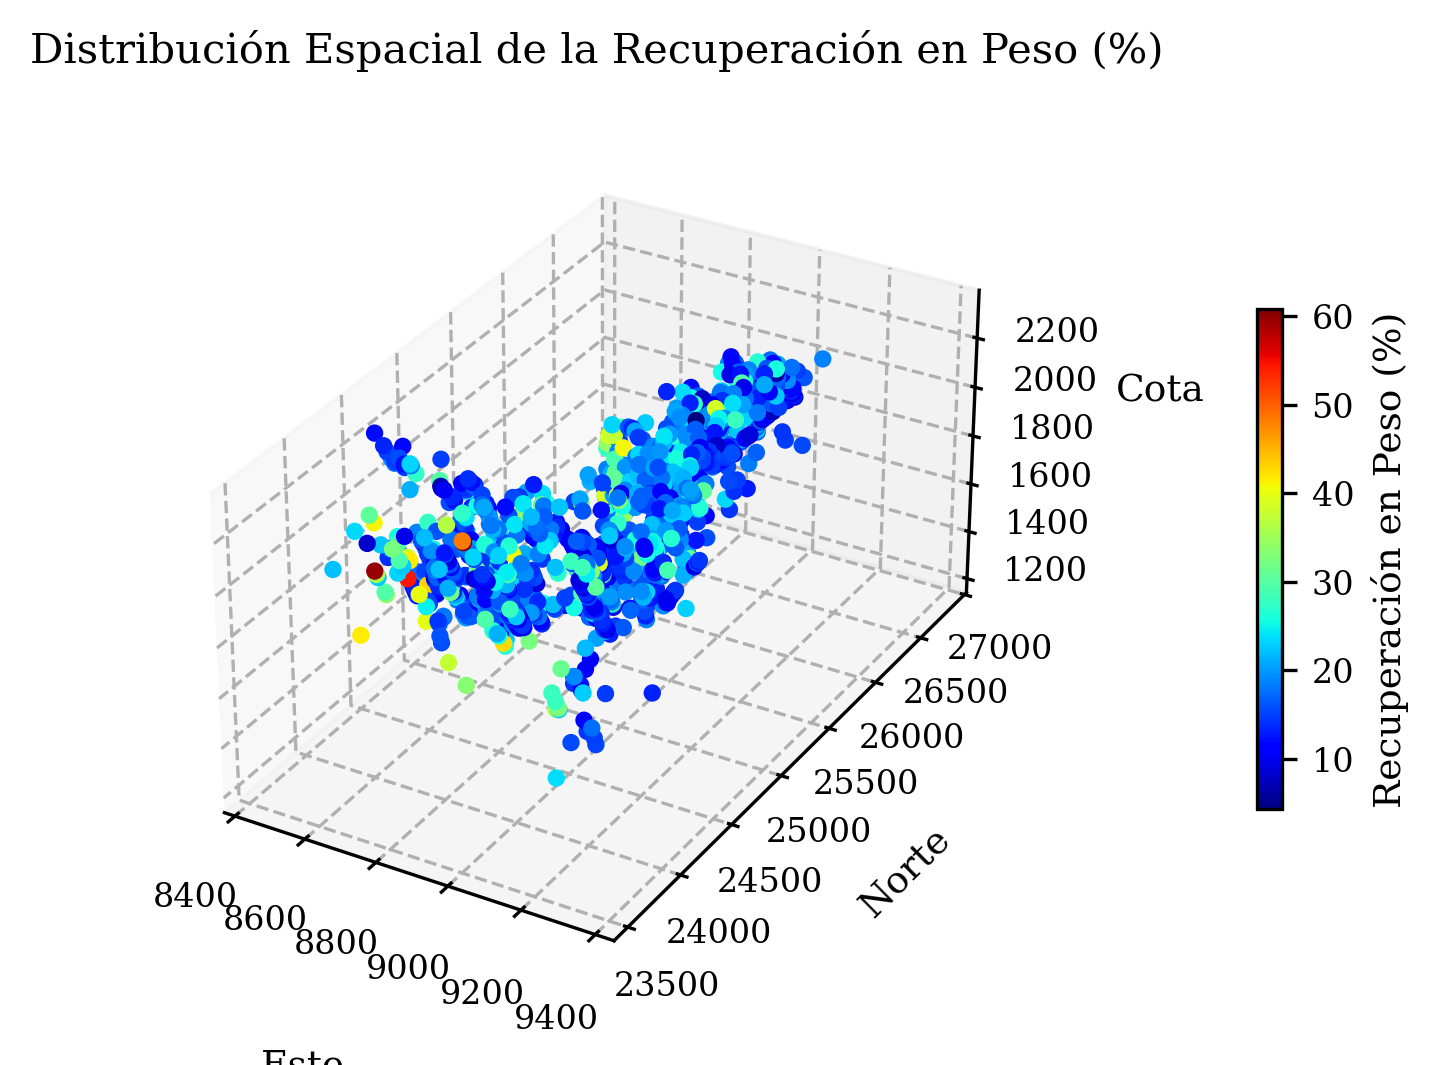
\includegraphics[width=\textwidth]{Imagenes/mapa_3d_recpe.png}
			\end{column}
			\begin{column}{0.42\textwidth}
				\vspace{10pt}
				\textbf{Observaciones clave}\\[8pt]
				\begin{itemize}
					\item La mayoría de las muestras presenta recuperaciones \emp{inferiores al 21\%} (tonos azules)
					\item Valores altos aparecen de forma \hl{localizada} — no distribuidos aleatoriamente
					\item Esto confirma \emp{continuidad espacial} y justifica el uso de coordenadas como predictores
				\end{itemize}
			\end{column}
		\end{columns}
	\end{frame}
	
	\begin{frame}{Deriva espacial — tendencias macroscópicas}
		\begin{columns}[T]
			\begin{column}{0.62\textwidth}
				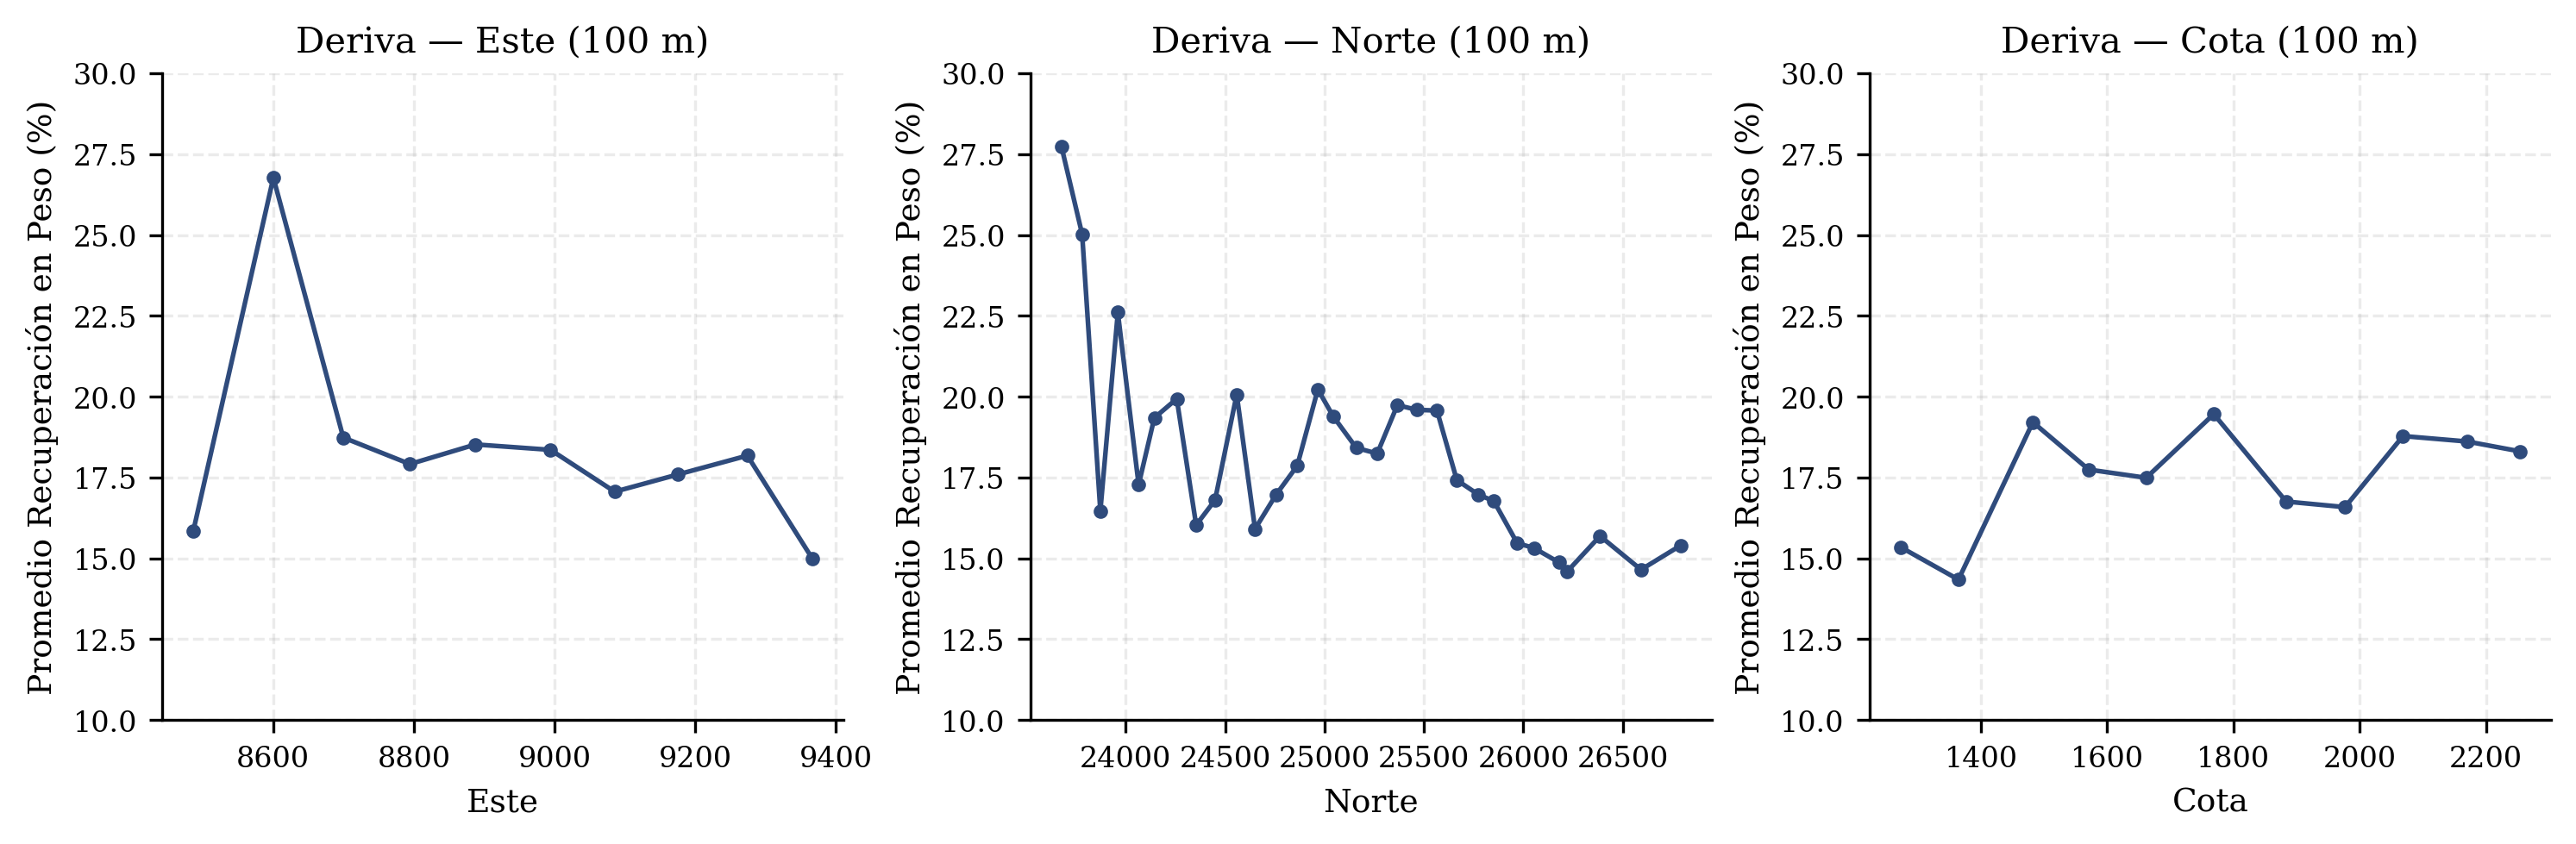
\includegraphics[width=\textwidth]{Imagenes/deriva_recpe.png}
			\end{column}
			\begin{column}{0.35\textwidth}
				\vspace{10pt}
				\textbf{Tendencias observadas}\\[8pt]
				\hl{Norte} — Caída progresiva desde\\
				$\sim$28\% (sur) hasta $\sim$15\% (norte)\\[8pt]
				\hl{Este} — Variaciones moderadas\\
				con peak en 8.600 m\\[8pt]
				\hl{Cota} — Comportamiento\\
				relativamente estable\\[10pt]
				\emp{La posición espacial es una\\
					variable predictora relevante.}
			\end{column}
		\end{columns}
	\end{frame}
	
	%=============================================================
	\section{Modelado: dominios con K-Means}
	%=============================================================
	
	\begin{frame}{Segmentación espacial con K-Means}
		\begin{columns}[T]
			\begin{column}{0.55\textwidth}
				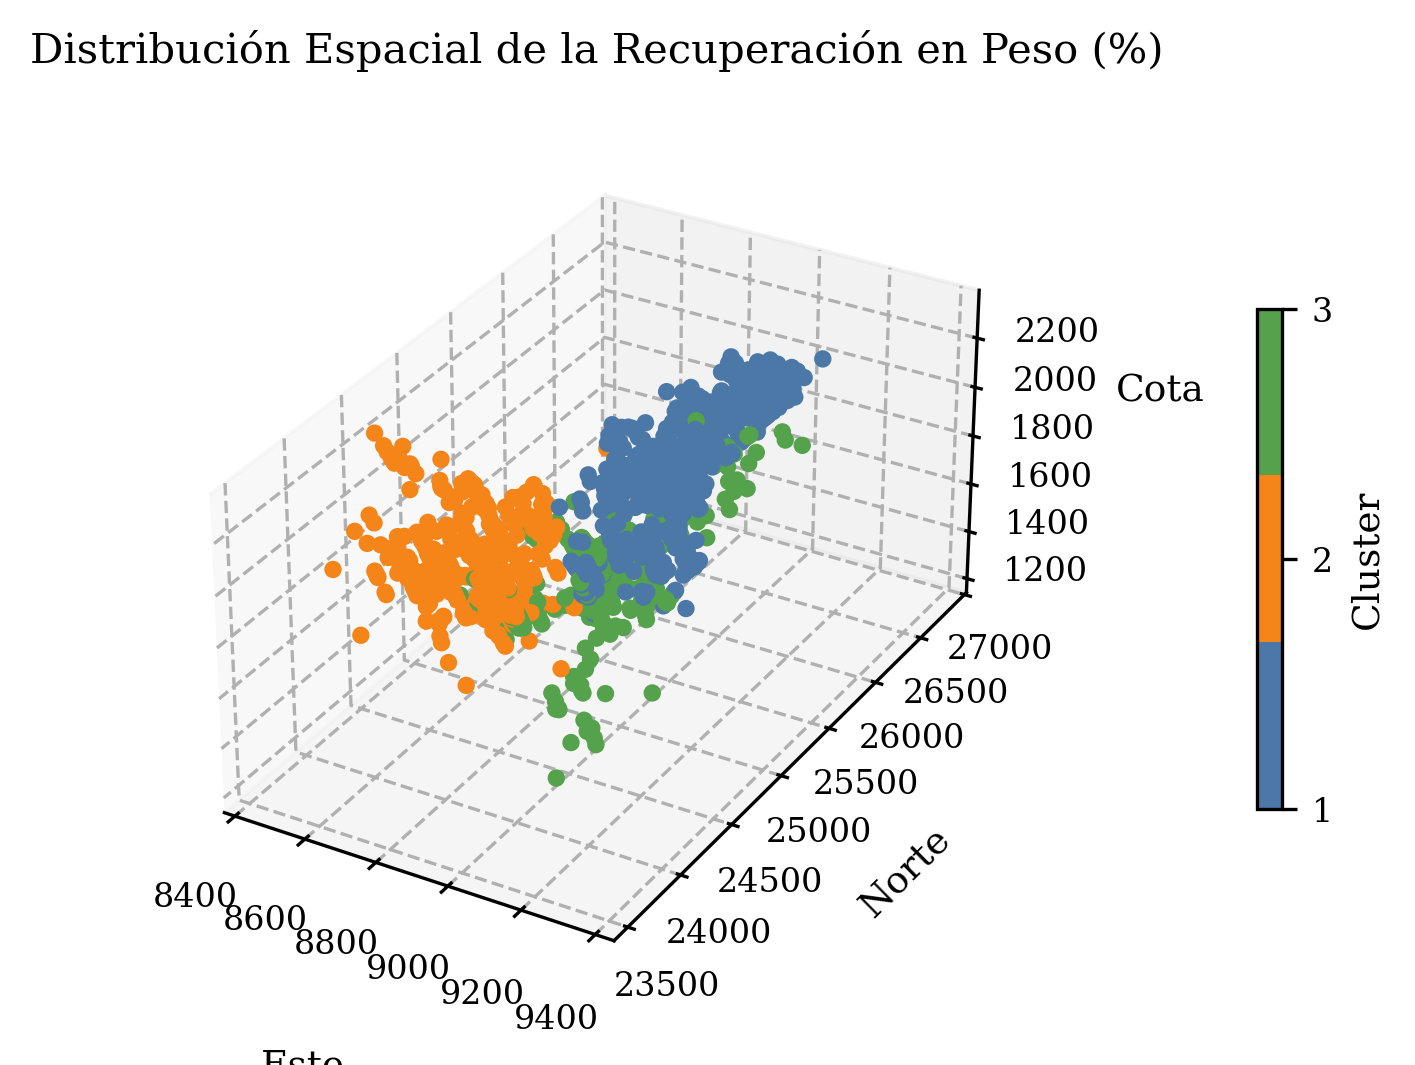
\includegraphics[width=\textwidth]{Imagenes/kmeans_clusters_3d.png}
			\end{column}
			\begin{column}{0.42\textwidth}
				\vspace{6pt}
				\textbf{Configuración}\\[4pt]
				Variables de entrada: coordenadas 3D\\
				+ recuperación en peso transformada\\[6pt]
				\textbf{3 clusters} — coincide con la\\
				segmentación del modelo de la empresa\\[10pt]
				
				\begin{tabular}{lcc}
					\toprule
					\textbf{Cluster} & \textbf{N} & \textbf{Media (\%)} \\
					\midrule
					1 & 580 & 18,74 \\
					2 & 371 & 19,56 \\
					3 & 268 & \hl{14,25} \\
					\bottomrule
				\end{tabular}\\[6pt]
				{\small Cluster 3 claramente diferenciado\\con menor recuperación y variabilidad.}
			\end{column}
		\end{columns}
	\end{frame}
	
	\begin{frame}{Comportamiento metalúrgico por cluster}
		\begin{columns}[T]
			\begin{column}{0.62\textwidth}
				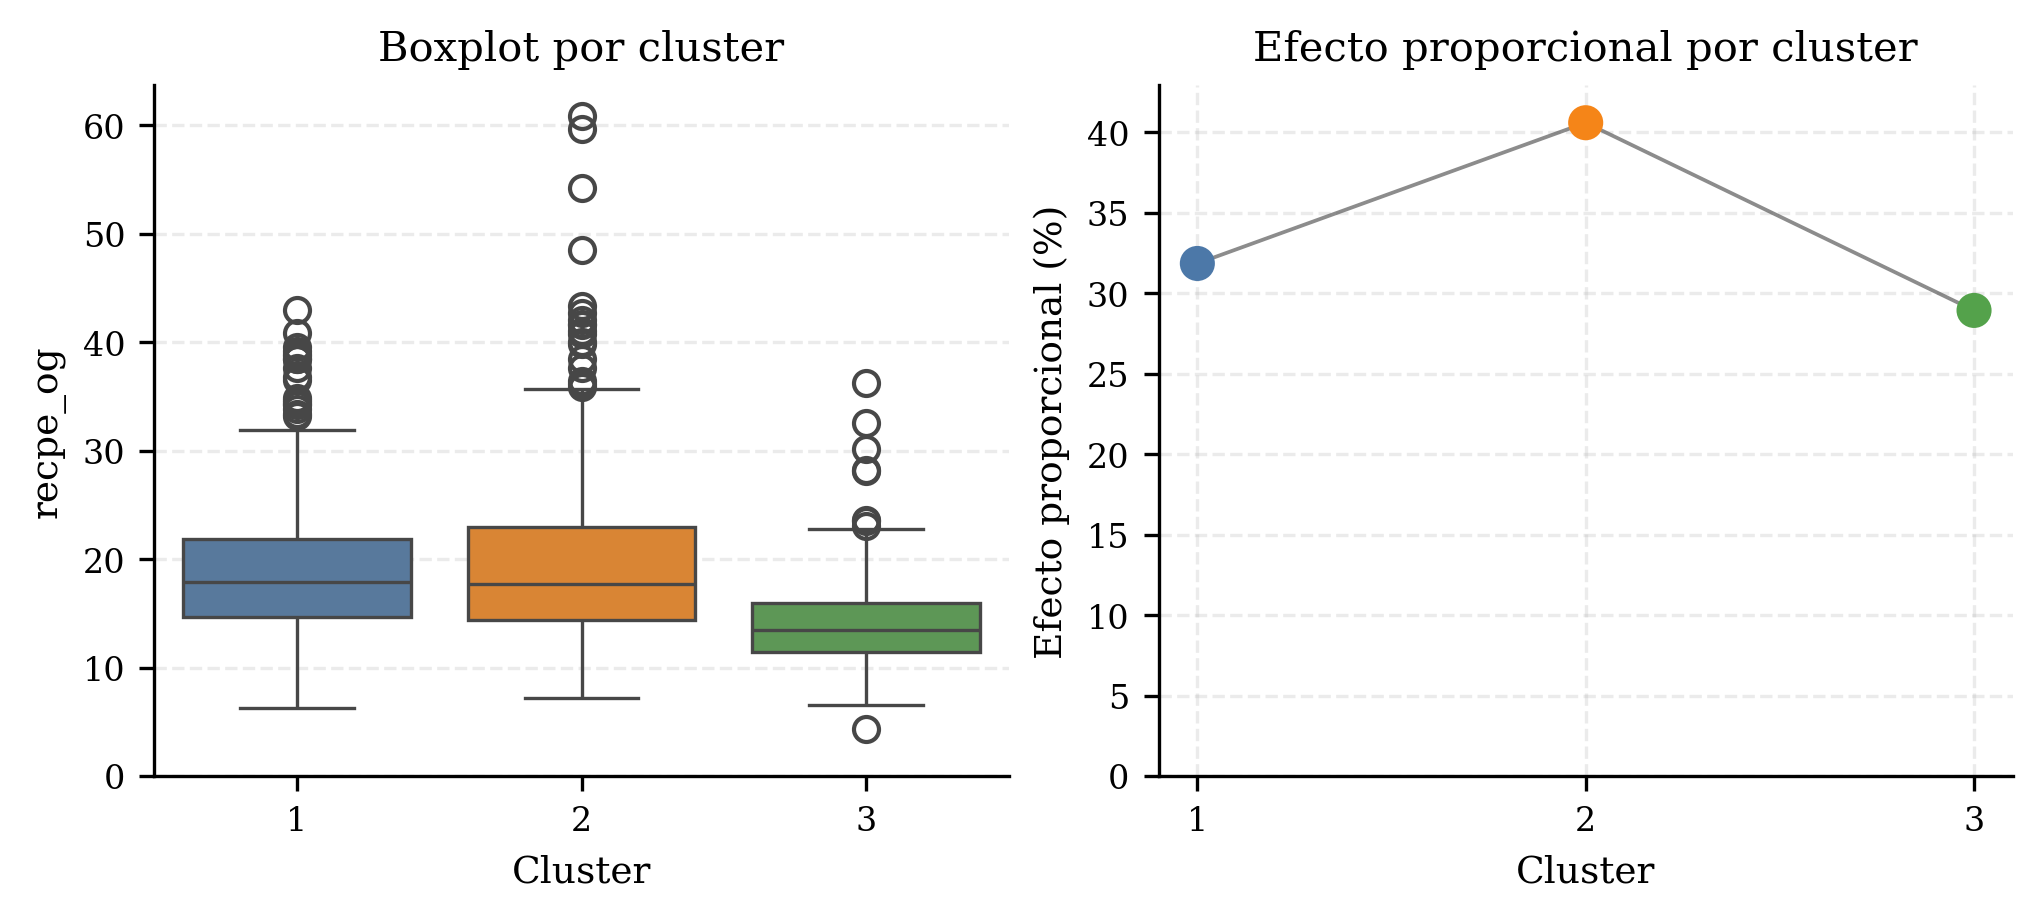
\includegraphics[width=\textwidth]{Imagenes/kmeans_clusters_boxplot_efecto_proporcional.png}
			\end{column}
			\begin{column}{0.35\textwidth}
				\vspace{10pt}
				\textbf{Interpretación}\\[8pt]
				\hl{Cluster 2} presenta el mayor\\
				efecto proporcional ($\sim$40\%):\\
				valores altos van acompañados\\
				de mayor variabilidad\\[8pt]
				\hl{Cluster 3} es el más homogéneo:\\
				recuperación baja y estable\\[8pt]
				Los tres grupos ocupan\\
				\emp{sectores distintos del yacimiento},\\
				validando la coherencia espacial\\
				de la segmentación.
			\end{column}
		\end{columns}
	\end{frame}
	
	%=============================================================
	\section{Modelado: ML vs Kriging}
	%=============================================================
	
	\begin{frame}{Métricas de desempeño}
		\begin{columns}[T]
			\begin{column}{0.48\textwidth}
				\vspace{6pt}
				Cuatro modelos entrenados con el \emp{100\% de los datos},\\
				validados externamente contra el modelo de bloques Kriging.\\[10pt]
				
				\begin{tabular}{lccc}
					\toprule
					\textbf{Modelo} & \textbf{R²} & \textbf{RMSE} & \textbf{MAPE} \\
					\midrule
					Kriging          & \hl{0,796} & \hl{2,992} & \hl{10,5\%} \\
					\midrule
					KNN              & 0,630 & 4,032 & 13,3\% \\
					Gradient Boost.  & 0,387 & 5,187 & 19,6\% \\
					XGBoost          & 0,364 & 5,282 & 20,0\% \\
					Random Forest    & 0,342 & 5,372 & 20,3\% \\
					\bottomrule
				\end{tabular}
			\end{column}
			\begin{column}{0.48\textwidth}
				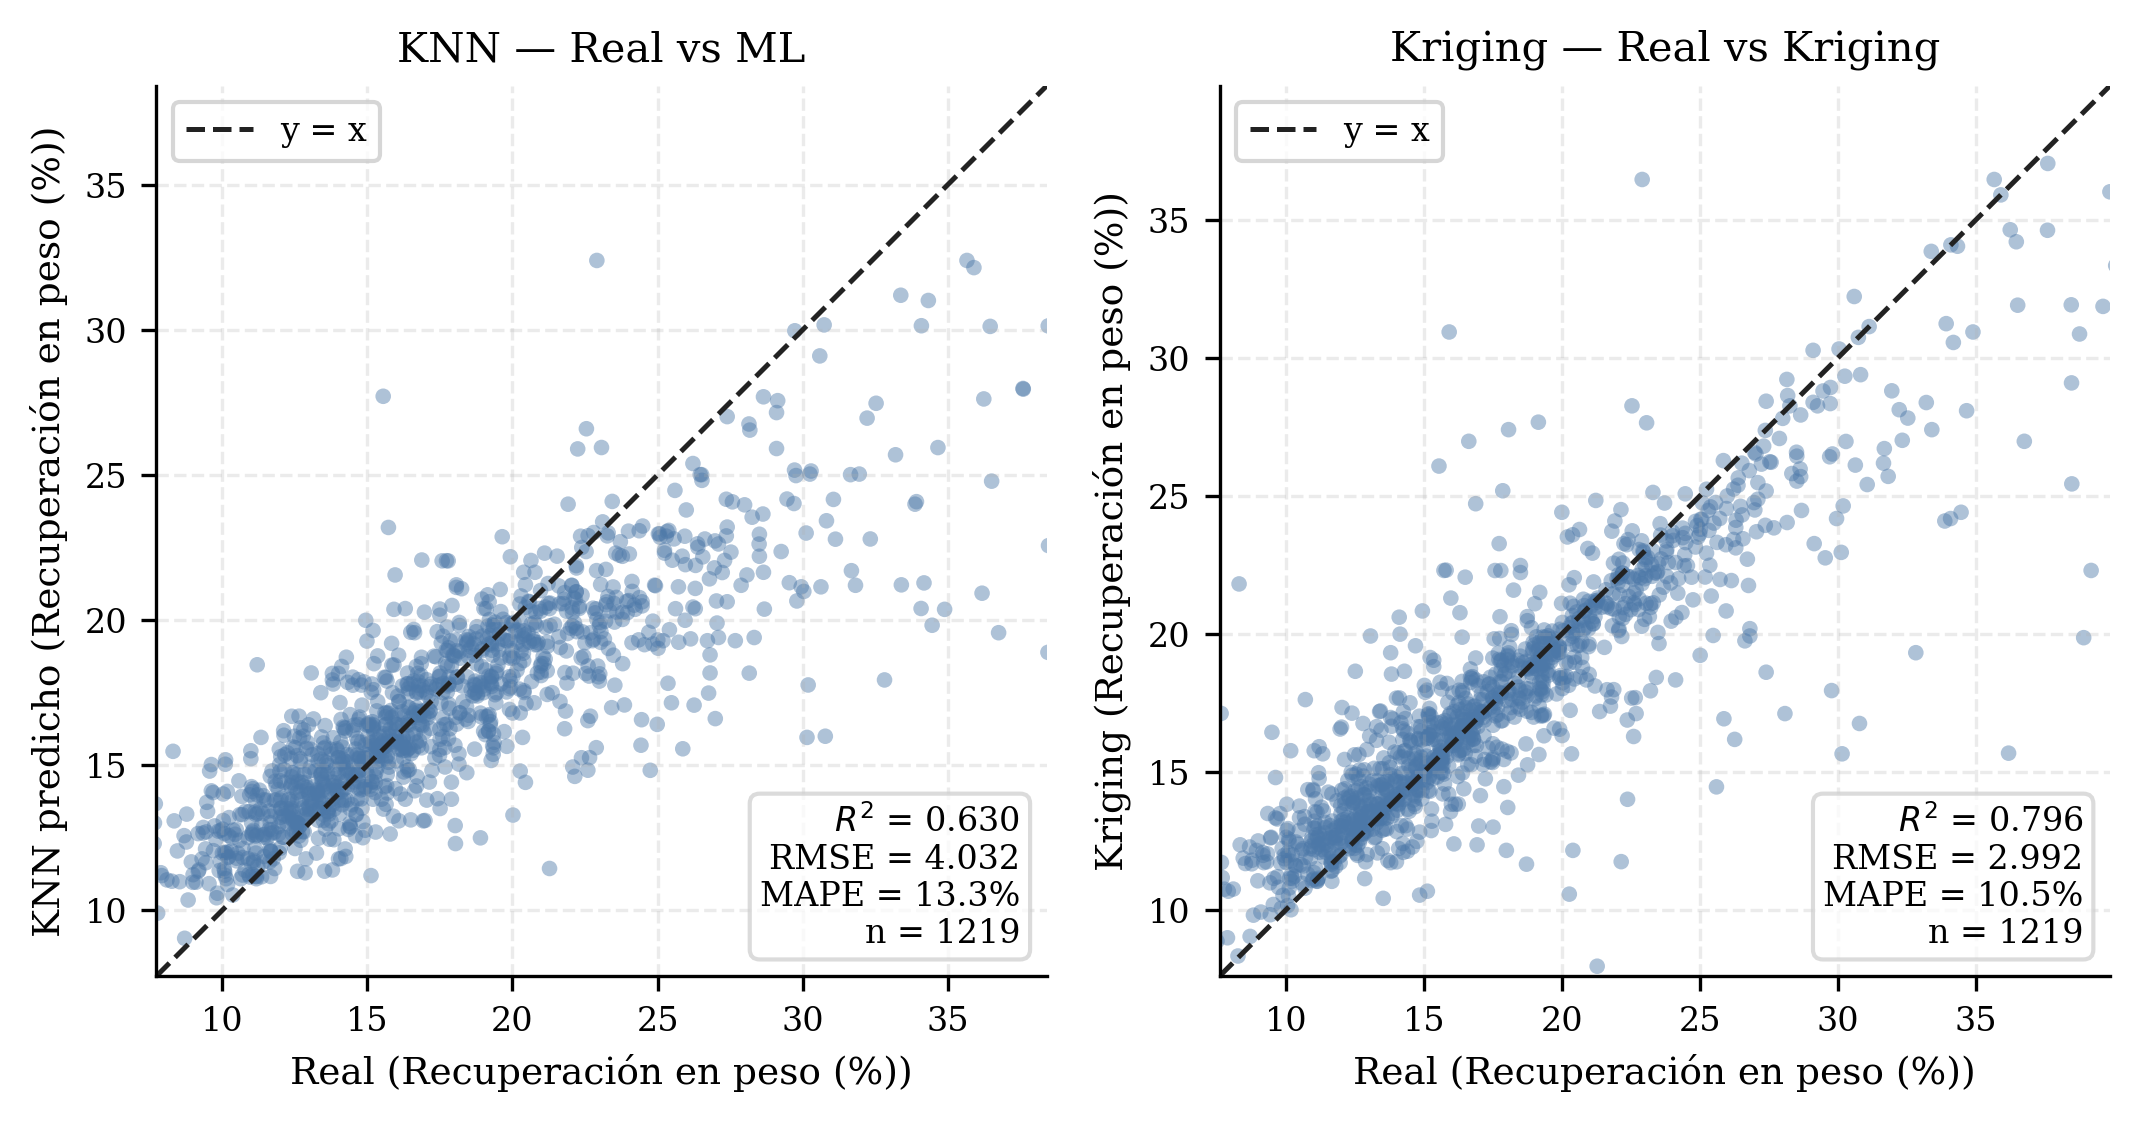
\includegraphics[width=\textwidth]{Imagenes/knn_vs_kriging.png}
			\end{column}
		\end{columns}
	\end{frame}
	
	\begin{frame}{Comparación de distribuciones}
		\begin{columns}[T]
			\begin{column}{0.60\textwidth}
				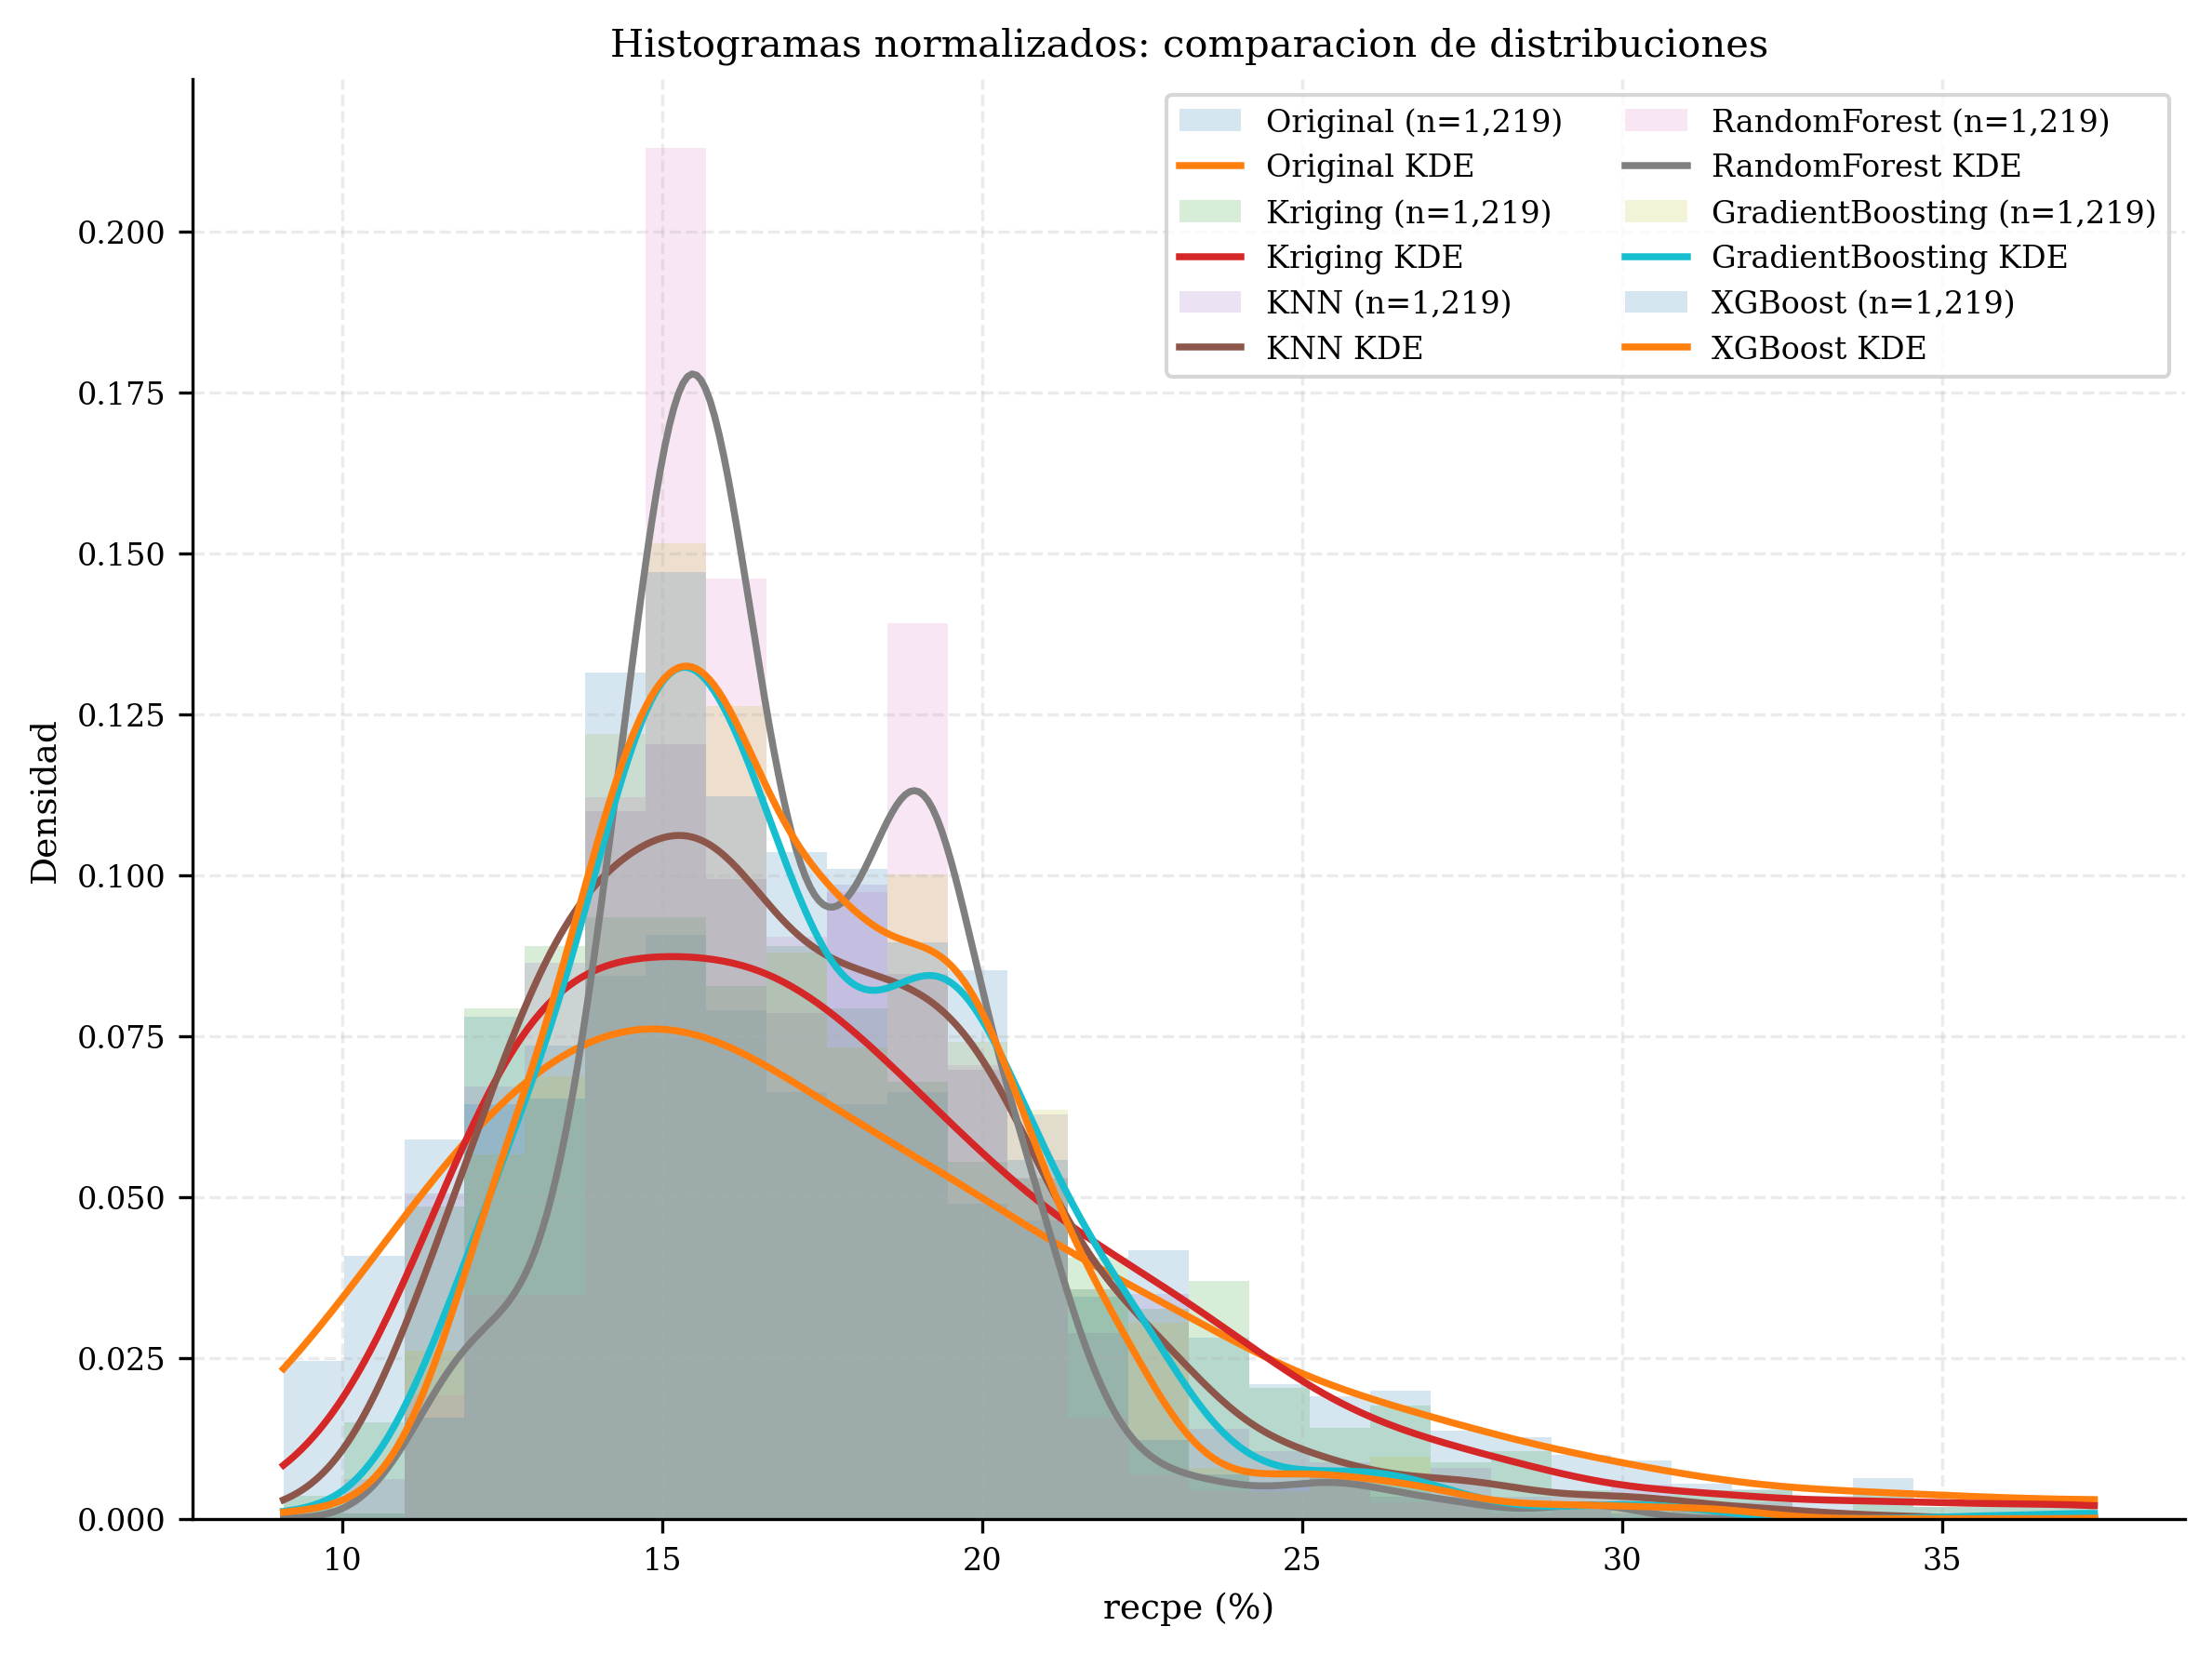
\includegraphics[width=\textwidth]{Imagenes/histogramas_normalizados.png}
			\end{column}
			\begin{column}{0.37\textwidth}
				\vspace{10pt}
				\textbf{Hallazgos}\\[8pt]
				\hl{KNN} reproduce mejor la forma\\
				general de la distribución original\\[8pt]
				\emp{Modelos de árboles} concentran\\
				sus predicciones en un rango más\\
				estrecho — pierden representatividad\\
				en los extremos\\[8pt]
				Kriging y KNN son los modelos\\
				con mejor \emp{fidelidad distribucional}
			\end{column}
		\end{columns}
	\end{frame}
	
	\begin{frame}{Coherencia espacial — Deriva dirección Norte}
		\begin{columns}[T]
			\begin{column}{0.62\textwidth}
				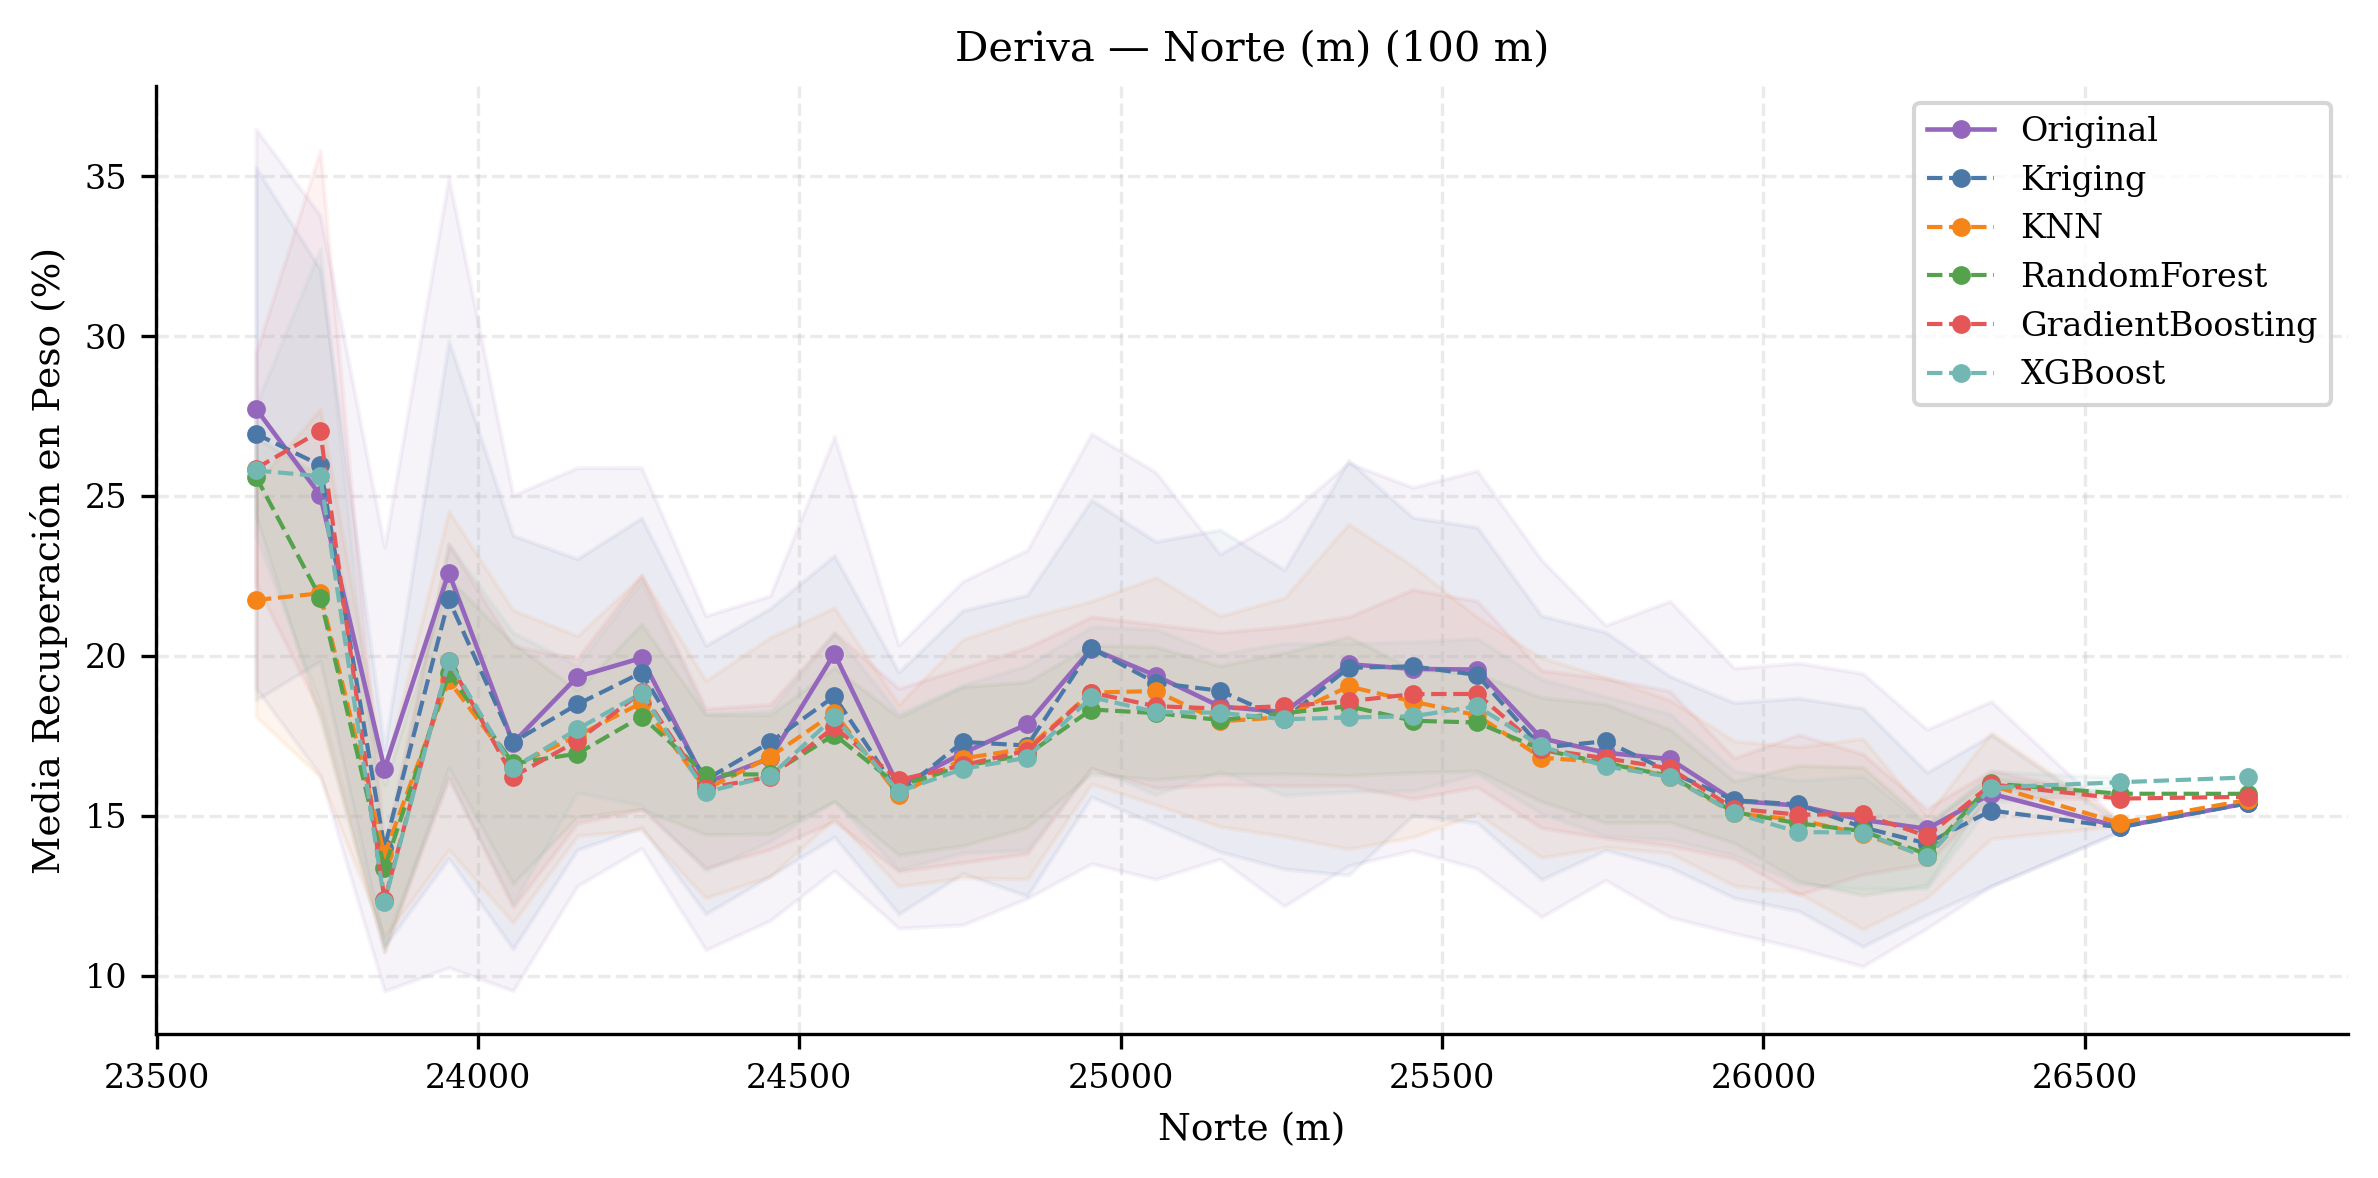
\includegraphics[width=\textwidth]{Imagenes/deriva_norte.png}
			\end{column}
			\begin{column}{0.35\textwidth}
				\vspace{10pt}
				\textbf{Todos los modelos}\\
				reproducen la tendencia\\
				global Norte-Sur\\[8pt]
				\hl{KNN y Kriging} siguen\\
				más de cerca la curva\\
				original en las 3 direcciones\\[8pt]
				\emp{Modelos de árboles}\\
				presentan mayor suavizado\\
				y pierden variaciones locales,\\
				especialmente en dirección Este
			\end{column}
		\end{columns}
	\end{frame}
	
	%=============================================================
	\section{Interpretación de resultados}
	%=============================================================
	
	\begin{frame}{¿Por qué KNN es el mejor modelo ML?}
		\begin{columns}[T]
			\begin{column}{0.48\textwidth}
				\begin{block}{Ventaja estructural de KNN}
					Configurado con \texttt{weights="distance"}:\\
					los vecinos más cercanos tienen\\
					mayor influencia en la predicción.\\[6pt]
					Distancia promedio entre puntos\\
					de validación y entrenamiento:\\
					\hl{$\approx$ 6,7 metros}\\[6pt]
					KNN es \emp{estructuralmente afín}\\
					a la lógica de interpolación espacial.
				\end{block}
			\end{column}
			\begin{column}{0.48\textwidth}
				\begin{alertblock}{¿Por qué fallan los árboles?}
					Random Forest, Gradient Boosting y\\
					XGBoost aprenden particionando el\\
					espacio en \textbf{regiones rectangulares}.\\[6pt]
					Esto les dificulta capturar la\\
					\textbf{continuidad espacial gradual}\\
					que caracteriza a un yacimiento.
				\end{alertblock}
			\end{column}
		\end{columns}
	\end{frame}
	
	\begin{frame}{La brecha KNN–Kriging en contexto}
		\begin{columns}[T]
			\begin{column}{0.48\textwidth}
				\textbf{Kriging de la empresa}\\[4pt]
				\begin{itemize}
					\item Construido por especialistas con experiencia en el yacimiento
					\item Parámetros variográficos ajustados manualmente
					\item Proceso que puede tomar \emp{semanas}
					\item Requiere \emp{software propietario de alto costo}
				\end{itemize}
			\end{column}
			\begin{column}{0.48\textwidth}
				\textbf{MVP desarrollado en esta tesina}\\[4pt]
				\begin{itemize}
					\item Pipeline automatizado en Python
					\item Sin conocimiento experto especializado
					\item Resultados en \hl{minutos}
					\item \hl{Código abierto}, sin licencias
				\end{itemize}
				\vspace{10pt}
				\begin{alertblock}{Conclusión}
					Un $R^2$ de \textbf{0,630} frente al \textbf{0,796}
					del Kriging es un resultado \hl{aceptable
						y prometedor} considerando la diferencia
					en esfuerzo y recursos.
				\end{alertblock}
			\end{column}
		\end{columns}
	\end{frame}
	
	%=============================================================
	\section{Conclusiones y trabajo futuro}
	%=============================================================
	
	\begin{frame}{Conclusiones}
		\begin{columns}[T]
			\begin{column}{0.48\textwidth}
				\textbf{Resultados principales}\\[6pt]
				\begin{itemize}
					\item La aproximación con ML es \hl{viable}
					\item KNN alcanzó $R^2 = 0{,}630$ vs $0{,}796$ del Kriging
					\item K-Means generó dominios con \emp{coherencia espacial y metalúrgica}
					\item Todos los modelos reproducen las \emp{tendencias espaciales globales}
					\item El MVP entrega estimaciones en \hl{minutos}, sin software propietario
				\end{itemize}
			\end{column}
			\begin{column}{0.48\textwidth}
				\textbf{Trabajo futuro}\\[6pt]
				\begin{enumerate}
					\item Incorporar variables geológicas y geometalúrgicas adicionales como predictores
					\item Explorar modelos diseñados específicamente para datos espaciales
					\item Aplicar validación cruzada que respete la correlación geográfica
					\item Integrar el pipeline al flujo oficial de estimación de recursos
				\end{enumerate}
			\end{column}
		\end{columns}
	\end{frame}
	
	\begin{frame}[standout]
		\Huge\textbf{¿Preguntas?}\\[12pt]
		\normalsize
		Ignacio Enrique Rojas Rodríguez\\[4pt]
		Magíster en Ciencia de Datos para la Innovación\\
		Universidad de Concepción — Marzo 2026
	\end{frame}
	
\end{document}